\documentclass[xcolor=table]{beamer}
\usepackage{beamerthemesplit}
\usepackage{wrapfig}
\usetheme{SPbGU}
\usepackage{pdfpages}
\usepackage{amsmath}
\usepackage{cmap} 
\usepackage[T2A]{fontenc} 
\usepackage[utf8]{inputenc}
\usepackage[english,russian]{babel}
\usepackage{indentfirst}
\usepackage{tikz}
\usepackage{multirow}
\usepackage[noend]{algpseudocode}
\usepackage{algorithm}
\usepackage{algorithmicx}
\usetikzlibrary{shapes,arrows}
%usepackage{fancyvrb}
%\usepackage{minted}
%\usepackage{verbments}


\newtheorem{rutheorem}{Теорема}
\newtheorem{ruproof}{Доказательство}
\newtheorem{rudefinition}{Определение}
\newtheorem{rulemma}{Лемма}
\beamertemplatenavigationsymbolsempty

\title[Brahma.FSharp]{Brahma.FSharp как средство ``прозрачного'' использования GPGPU в программах на F\#}
%\subtitle[YaccConstructor]{Parsing techniques for graph analysis}
% То, что в квадратных скобках, отображается в левом нижнем углу. 
\institute[СПбГУ]{
JetBrains Research, лаборатория языковых инструментов \\
Санкт-Петербургский государственный университет
}

% То, что в квадратных скобках, отображается в левом нижнем углу.
\author[Семён Григорьев]{Семён Григорьев}

\date{30.11.2017}

\definecolor{orange}{RGB}{179,36,31}

\begin{document}
{
\begin{frame}[fragile]
  \begin{tabular}{p{2.5cm} p{6.5cm} p{2cm}}
   \begin{center}
      
\includegraphics[height=1.5cm]{pictures/JBLogo3.pdf}
    \end{center}
    &
    \begin{center}
      
\includegraphics[height=1.5cm]{pictures/fprog_logo.png}
    \end{center} 
    &
    \begin{center}
      
\includegraphics[height=1.5cm]{pictures/SPbGU_Logo.png}
    \end{center}
  \end{tabular}
  \titlepage
\end{frame}
}


\begin{frame}[fragile]
  \transwipe[direction=90]
  \frametitle{Введение: GPGPU}
  \begin{itemize}
  \item GPGPU --- General-purpose computing for graphics processing units
    \begin{itemize}
        \item Реализация SIMD --- одна инструкция применяется ко многим данным
        \item Массовый параллелизм общего назначения
    \end{itemize}
    \end{itemize}
    \begin{center}
      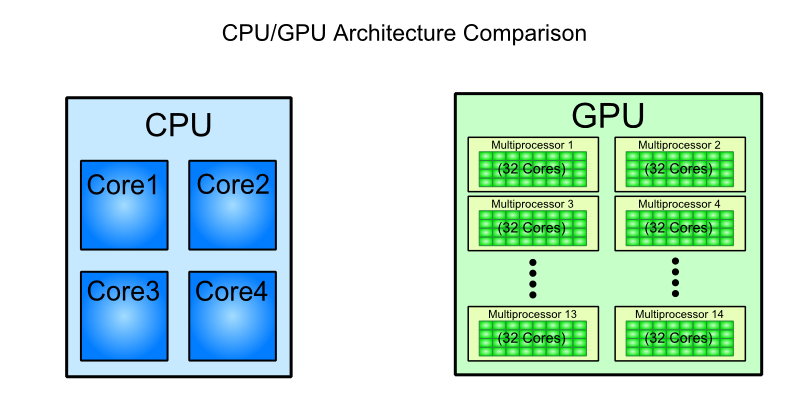
\includegraphics[width=0.7\textwidth]{pictures/cpu_vs_gpu.png}\footnote{\small{http://blog.goldenhelix.com/wp-content/uploads/2010/10/cpu\_vs\_gpu.png}}
    \end{center} 
\end{frame}

\begin{frame}[fragile]
  \transwipe[direction=90]
  \frametitle{Введение: Техники реализации GPGPU}
    \begin{itemize}
        \item CUDA
        \item \textbf{OpenCL}
        \item OpenACC
        \item C++ AMP
        \item ...
    \end{itemize}        
\end{frame}

\begin{frame}[fragile]
  \transwipe[direction=90]
  \frametitle{План}
  \begin{itemize}
  \item GPGPU в F\#: но зачем?
    \begin{itemize}
        \item Есть ли будущее у таких решений?
        \item Где их можно применять?
    \end{itemize}
  \item Почему именно так, а не инече?
      \begin{itemize}
        \item Уместен ли такой подход?
        \item Может можно проще?
      \end{itemize}
   \item Что под капотом у Brahma.FSharp?
  \end{itemize}
\end{frame}

\begin{frame}[fragile]
  \transwipe[direction=90]
  \frametitle{Зачем и почему GPGPU?}
  \begin{itemize}
  \item Обработка больших объёмов данных ``регулярным'' способом
    \begin{itemize}
        \item Аналитика
        \item Моделирование
        \item ...
        \item BigData
    \end{itemize}
  \item Вычислительные возможности растут
    \begin{itemize}
        \item Тысячи ядер
        \item Гигабайты оперативной мамяти
        \item Динамический параллелизм
    \end{itemize}
    \end{itemize}
\end{frame}

\begin{frame}[fragile]
  \transwipe[direction=90]
  \frametitle{Модель мира OpenCL}
    \begin{center}
      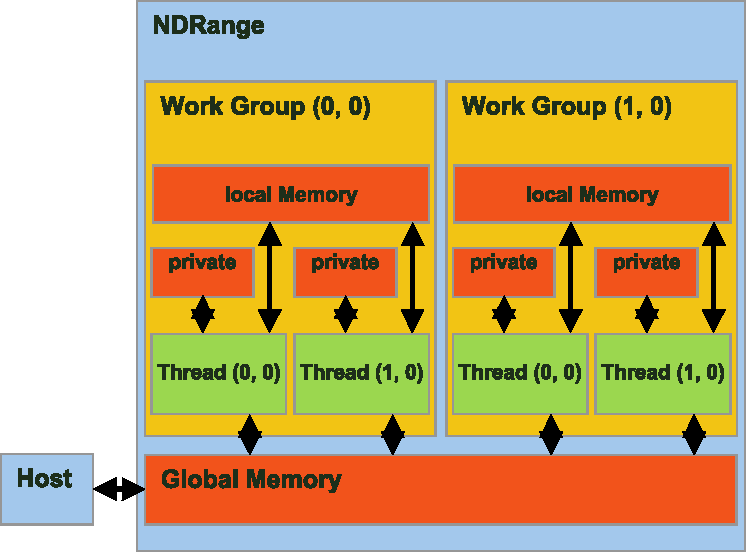
\includegraphics[width=0.8\textwidth]{pictures/Model1.pdf}\footnote{\small{Wen-mei Hwu and John Stone, ``The OpenCL Programming Model''}}
    \end{center} 
\end{frame}


\begin{frame}[fragile]
  \transwipe[direction=90]
  \frametitle{Модель мира OpenCL}
    \begin{center}
      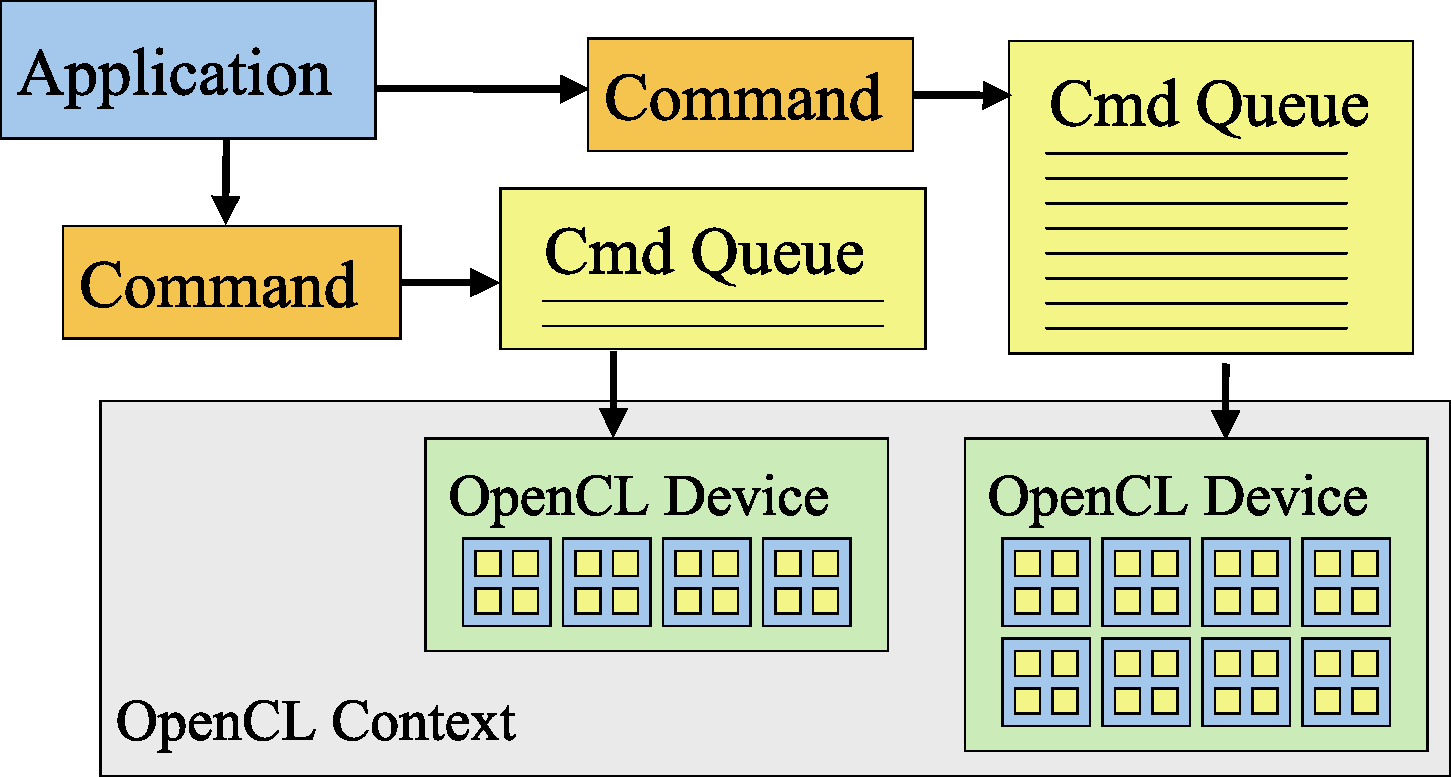
\includegraphics[width=0.9\textwidth]{pictures/Model2.pdf}\footnote{\small{Wen-mei Hwu and John Stone, ``The OpenCL Programming Model''}}
    \end{center} 
\end{frame}


\begin{frame}[fragile]
  \transwipe[direction=90]
  \frametitle{Доступ к GPGPU из .NET}
  \begin{itemize}
  \item Средства программирования видеопроцессоров в .NET
  \begin{itemize}
     \item Alea GPU (CUDA)
     \item Brahma.FSharp (OpenCL)
     \item FSCL (OpenCL)
  \end{itemize}
  \item Средства запуска CUDA-кода из ЯВУ:
  \begin{itemize}
     \item CUSP
     \item ManagedCuda
  \end{itemize}
  \item ``Низкоуровневые драйвера''
  \begin{itemize}
     \item OpenCL.NET
     \item CUDA.NET
  \end{itemize}
  \end{itemize}
\end{frame}


\begin{frame}[fragile]
  \transwipe[direction=90]
  \frametitle{Почему именно так, а не инече?}
      \begin{itemize}
        \item ``Надёжность'' --- использование системы типов F\# и других особенностей языка и компилятора
        \item ``Прозрачность''/гомогенность разработки для гетерогенных систем
      \end{itemize}
\end{frame}

\begin{frame}[fragile]
  \transwipe[direction=90]
  \frametitle{Провайдеры типов}
  \begin {itemize}
  \item Функция построения типа по пользовательскому контексту
  \item Преимущества перед кодогенерацией
  \begin {itemize}
   \item Интеграция с пользовательским контекстом
   \item Статическая типизация
   \item Вспомогательная информация доступна в процессе разработки (работает автодополнение и т.д.)
  \end {itemize}

  \item Недостатки
  \begin {itemize}
    \item Высокая сложность тестирования
    \item Высокая сложность отладки
  \end {itemize}
  \item Помощь трудящимся: FSharp.TypeProviders.SDK (\url{https://github.com/fsprojects/FSharp.TypeProviders.SDK})
\end {itemize}
\end{frame}

\begin{frame}[fragile]
  \transwipe[direction=90]
  \frametitle{Цитирование кода (Code quotation)}
  \begin{itemize}
  \item \url{https://docs.microsoft.com/en-us/dotnet/fsharp/language-reference/code-quotations}
  \item Предоставление доступа к дереву разбора F\#-кода во время выполнения
  \end{itemize}
\end{frame}

\begin{frame}
  \transwipe[direction=90]
  \frametitle{Что дальше?}
\begin{itemize} 
\item Расширение возможностей транслятора
\item Улучшение управления памятью
\item Смешанные вычисления
\item Использование возможностей F\# для параллельного/асинхронного программирования
\begin{itemize} 
  \item MailboxProcessor
  \item Hopac
  \item ...
\end{itemize}
\end{itemize}

\end{frame}

\begin{frame}
  \transwipe[direction=90]
  \frametitle{Итоги}
\begin{itemize} 
\item Есть ли будущее у такого подхода?
\begin{itemize} 
  \item Какие альтернативы?
  \item Нужна ли гомогенность?
  \item ...
\end{itemize}
\item Какие потенциальные области применения?

\end{itemize}

\end{frame}

            
\begin{frame}
\transwipe[direction=90]
\frametitle{Контакты}
\begin{itemize}
  \item Почта: \url{semen.grigorev@jetbrains.com}
  \item Проект на GitHub: \url{https://github.com/YaccConstructor/Brahma.FSharp}
\end{itemize}
\end{frame}
\end{document}
